\documentclass[mscthesis]{usiinfthesis}
\usepackage{lipsum}


\usepackage{listings}
\graphicspath{ {./figures/} }

\lstdefinelanguage{algebra}
{morekeywords={import,sort,constructors,observers,transformers,axioms,if,
else,end},
sensitive=false,
morecomment=[l]{//s},
}

% Variables
\newcommand\numberevents{59256 }

% For equations float
\usepackage{float}
\usepackage{aliascnt}
\newaliascnt{eqfloat}{equation}
\newfloat{eqfloat}{h}{eqflts}
\floatname{eqfloat}{Equation}

\newcommand*{\ORGeqfloat}{}
\let\ORGeqfloat\eqfloat
\def\eqfloat{%
  \let\ORIGINALcaption\caption
  \def\caption{%
    \addtocounter{equation}{-1}%
    \ORIGINALcaption
  }%
  \ORGeqfloat
}


\title{Alien species modelling via relational event models} %compulsory
%\specialization{Dependable Distributed Systems}%optional
%\subtitle{Subtitle: Reinventing the World} %optional 
\author{Niccol\`o Zuppichini} %compulsory
\begin{committee}
\advisor{Prof.}{Ernst-Jan Camiel}{Wit} %compulsory
\coadvisor{Prof.}{Igor}{Artico}{} %optional
\end{committee}
\Day{15} %compulsory
\Month{June} %compulsory
\Year{2022} %compulsory, put only the year
\place{Lugano} %compulsory

\dedication{To my beloved} %optional
\openepigraph{Someone said \dots}{Someone} %optional

%\makeindex %optional, also comment out \theindex at the end

\begin{document}

\maketitle %generates the titlepage, this is FIXED

\frontmatter %generates the frontmatter, this is FIXED

\begin{abstract}
% Topic introduction
During the last centuries human research on the interaction of species substantially intensified. However, we know little to nothing about the underlying process that shape the behaviours of alien species invasion across regions, countries and ecosystems.

% What we do here
In this paper we present a custom relational event model to study the the invasion of alien species, which are that are abnormally found outside of their native land. We describe the invasion of species as a temporal unidirectional bipartite species-region graph. Under this framework, We present a relation event model to model the study of co-invasion of species. We then apply this model to a subset of the dataset of \numberevents events ranging from (TODO years dataset). The aim of this paper is hence to study what group of species have the tendency to co-invade a region
.
g
% What we got
Using years of first records of (number) invasion of alien species from (number) taxonomic groups we show how a custom relational event model can be used to model the dynamics of species invasion. Due to the high size of the dataset, we also present an high performance implementation in python of our model.

%TODO should I put reference in introduction?
%TODO should I tak briefly about previous research?
%TODO introduce briefly computational challenge and HPC

\end{abstract}

%\begin{acknowledgements}
%\lipsum 
%\end{acknowledgements}

%\tableofcontents 
%\listoffigures %optional
%\listoftables %optional

\mainmatter

\chapter{Introduction}
% 1. Motivation. Why invasive species are a problem?
% 2. Briefly introduce the dataset
% 3. Briefly introduce how I will study the dataset
% 4. Briefly introduce how I will study the dataset
% 5. TODO briefly report the results

The rate at which alien species invade countries have increased over the last century and it's becoming an issue. The economic impact of alien species in Europe is estimated to be close to 13 billion dollars annually (\citet{intro:rate}). The interest in the study of the dynamics of alien species has been increasing over the years for this reason. Unfortunately, due to the complexity of the problem, is hard to come up with real actions. Intuitively, the invasion rate of species differs belonging to different taxonomic groups, however, a comprehensive global invasion dynamics study of the last centuries subdivided by taxonomic groups is still lacking. The dynamics of invasive species are driven by a multitude of factors simultaneously. These factors can be complex involving exogenous, endogenous, sociological, ecological and socio-economic factors. (\citet{intro:factors}). Given the complexity of the subject, it's important to develop a framework capable of studying and analyzing all the underlying effects simultaneously. 

Relational event modelling was first developed in the field of social network analysis (\citet{rem:butts}). A relational event is an interaction between a sender and a receiver at a specific timestamp. A relational event model studies the temporal sequence of such relational events. This framework has many advantages in the fact that it's able to study underlying temporal patterns, can efficiently deal with time-varying variables and it's a suitable diagnostic tool to test a hypothesis model on actual data. Due to its versatility, it was then applied in a large number of different fields such as animal-animal interaction (\citet{intro:cattle}), TODO cite 2 more.

%%TODO what did other people do?
%In the years, there have been a large number of different statistical approaches to relation event models to predict the appearance and spread of alien species.  
%
%%TODO review this
%To tackle the problem a dataset containing an extensive amount of invasive species in multiple geographic regions worldwide.  has been created (\citet{intro:dataset}). To further extend this study \citet{intro:ecological} fitted a REM on the dataset. \\
%%TODO I can't find the "Analysing ecological dynamics with relational event
%%models: the case of invasion events" paper

In this paper, we introduce a novel custom relational event model to study the dynamics of co-invasion of species in a latent space. The model takes into consideration multiple species simultaneously and studies the underlying relationship between different species co-invading regions by training on the most exhaustive source of first records of alien species in multiple regions in the world (TODO add ref). By studying the proximity of species and regions in the latent space, our model is capable of determining the group of species that have the tendency to co-invade a region and, in an analogous way, the group of regions that are more likely to be invaded by the same group of species.

% Structure of the thesis
In chapter 2 we present an exaustive statistical background of the methods used for the reader. In chapter 3 we make a preliminary study of the  dataset of the alien species, provide a formulation of our latent space relational event model and propose an efficient algorithm to make inferences about the latent space. In chapter 4 we discuss implementation specifications and frameworks used. In chapter 5 we present our results by applying our model to the dataset. In chapter 5 we discuss our result.

\chapter{Background}
\section{Relational event models (REM)}

Butts (\citet{rem:butts}) proposed a statistical modeling framework capable of analysing temporal information and evolution of a sequence of relational events. Given a set of receiver nodes, a set of sender nodes and a timeframe, a relational event \textit{e} is a triplet of a sender, a receiver and a timestamp. Depending on the underlying data, the sender set and receiver set may be disjoint to represent relationships. As instance, for studying the interaction between domestic animals the sender and receiver nodes belong to the same set (\citep{intro:cattle}). In contrast, when studying alien species invasion the species are the senders, the regions the receivers and they belong in disjoint sets. In general, a REM specifies time-varying event-rates for all dyads as a function of past events $E=(e_1, ..., e_N)$ where each event $e_i$ is defined as

\[
e_i = (s_i, r_i, t_i)
\]

In the above notation, $s_i \in S_{t_i} $ is the sender node, $r_i \in R_{t_i}$ the receiver node and $t_i$ is the time of the interaction. The sets $S_t, R_t$ respectively contain all the receiver and senders nodes at the current timestep $t_i$. The cross product of these two sets is called \textit{risk set} $R_{t_i}$  \footnote{\label{riskset_footnote}To avoid confusion, note that Butts originally called this set the \textit{support set}.}



\[
R_{t_i} = S_{t_i} \times R_{t_i}
\]

The risk set is the set of all dyads for which an event $e_{t_i}$ may occurr, hence, any relation event at time $t_i$ belongs to the risk set.

\[
\forall e_{i} \in R_{t_i}
\]

The hazard function $\lambda$ is defined as

%TODO you can write the formula better using REM_02 notes
\[
\lambda(s, r, t) = \lim_{\delta T \lim 0} \frac{P(t \leq T \leq t + \delta t | t \leq T}{\delta t}
\]

With some ease, the hazard function can be interpreted as the expected number of relational events in a time interval of lenght one, conditionally on the previous network events. The most common used hazard function is the Cox proportional hazard model. 

%TODO Theta is what we usually called beta (change it?)

\[
\lambda(s, r, t|G, \theta) = \lambda_0(t) \cdot \lambda_1(s, r, t|G, \theta)
\]
\[
\lambda_1(s, r, t|G, \theta) = exp(\sum_{j=1}^k \theta_j \cdot p_j(s, r|G)
\]

In this equation, $\lambda_0$ represents a baseline harzard for all dyads in the risk set - the function $\lambda_1$ is the propability that an event at $t$ happens between a node $s$ and a node $r$. To estimate the parameters $\theta$ we maximise the partial likelihood of the Cox proportional hazard model 

\[
L(\lambda) =  \prod_{e \in E} \frac{\lambda_1(s_i, r_i, t_i | G, \theta}{ \sum_{s \in R_{t_i}} \lambda_1(s, r, t_i | G, \theta}
\]



In a REM study we are generally interested in the factors that increase, or decrease, the hazard function.


\section{Extended Kalman Filter}

In 1960 R.E. Kalman published his paper describing a recursive solution to the discrete-data linear filtering problem (\citet{paper:kalmanfilter}). Since then, the Kalman filter gained extremely popularity in the machine learning and robotics resaerch field, particularly in area of autonomous navigation systems. The Kalman filter estimates the evolution of a process by using a feedback control. The filter first computes an estimation of the current proces state at some time, then, it tries to "filter out" the measurement  noise in a iterative process. As such, the Kalman filter equations can be subdivided into two categories: prediction step and update step. The prediction step is responsible for projecting forward in time the current state of the system. The update step takes the a-prior estimate given from the prediction step and by taking new measurements of the errror tries to obtain an improved a-posteriore estimate of the state. Indeed, the general form of the algorithm resembles a predictor-corrector algorithm for solving numerical problems. In this chapter I will provide a brief non-technical overview of the Kalman filter. A reader interested in a more in-depth discussion of the formulation of the Kalman filter is advised to read \citet{paper:Maybeck79}.

%A very “friendly” introduction to the
%general idea of the Kalman filter can be found in Chapter 1 of [Maybeck79], while a more complete
%introductory discussion can be found in [Sorenson70], which also contains some interesting
%historical narrative. More extensive references include [Gelb74], [Maybeck79], [Lewis86],
%[Brown92], and [Jacobs93].

\begin{figure}[h]
    \centering
    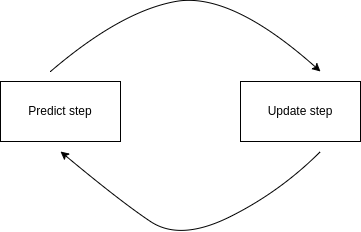
\includegraphics[width=0.25\textwidth]{kalman_diagram.png}
    \caption{The Kalman filter cycle. The time update forwards the current state estimate in time. The measurement update filters the noise out of the projected estimate.}
    \label{fig:kalman_cycle}
\end{figure}

Let's consider a non-linear system, $\epsilon$ captures uncertainity in the model, $v$ denotes the measurement noise. Both variables are white noises, random distributions with zero mean and uncorellated with the initial state $x_0$. The initial state $x_0$ is a random vector with known mean $\mu_0 = E[x_0]$ and variance $V_0 = E[(x_0-\mu_0)(x_0-\mu_0)^T]$.

\[
x_t = f(x_{t-1}) + \epsilon \; , \; \epsilon ~ N(0, \Sigma)
\]
\[
y_t = h(x_{t}) + v_{t} \; , \; \epsilon ~ N(0, \Delta)
\]

Providing that $f, y \in C^1$, we can linearize the process around the mean


We define $\hat{x}_t^-$ to be our a-priori estimate of the state $x$ at time $t$, given the knowledge of the previous state. Similarly, we define $\hat{x}_t$ to be our a-posteriori estimate at time $t$ given a measurement $y_t$. The goal of the Kalman filter is to express the a-posteriori state $\hat{x}_t^-$ in terms of a linear combination of the a-priori state and the difference an actual measurement $y$ and a measurement prediction $H\hat{x}_t^-$ state. 

\[
\hat{x}_t \in span(\hat{x}_t^-, y_t - H\hat{x}_t^-) 
\]
\[
\hat{x}_t = H\hat{x}_t^- + K (y_t - H_t \hat{x}_t^-)
\]

For a statistical motivation, I redirect the reader to \citet{paper:Maybeck79}. The difference $y_t - H_t \hat{x}_t^-$ is a residual of the estimation against the measurement, reflecting the error between the predicted measurement and the real measurement. The matrix $K$ is called Kalman gain matrix and is defined as 

\[
K_t = V_t^- H^T_t (H_t V_t^- H^T_t + R_t)^{-1} 
\]

The Kalman gain matrix goal is to minimise the a-posteriori covariance error matrix $V_t$ at time $t$. With some ease, a way of thinking $K$ is that as the measurement error covariance $R$ is close to zero the measurement $y$ is trusted more and the predicted measurement $H\hat{x}_t^-$ is on the other hand trusted less. On contrary, if the a-priori estimate error covariance $P^-$ is close to zero, the acual measurement $y$ is less trusted and the predicted meausrement $H\hat{x}_t^-$ trust is increased. The "trust" is then reflected into the weights of the Kalman gain matrix $K$. 

The initial state of the algorithm is given by

\begin{eqfloat}
\begin{equation}
\begin{array}{l}
\hat{x}_0 = \mu_0 = E[x_0] \\
\hat{V}_0 = V_0 = E[(x_0-\hat{x}_0)(x_0-\hat{x}_0)^T] 
\end{array}
\label{eq:kalman_init}
\end{equation}
\caption{Initialization}
\end{eqfloat}

We forecast an update of the estimation of $\hat{x} \approx x$

\begin{eqfloat}
\begin{equation}
\begin{array}{l}
\hat{x}_t^- = f(\hat{x}_{t-1}) \\
\hat{V}_t^- = J(x^f_{t-1}) V_{t-1} J(x^f_{t-1})^T + W_{t-1} Q_{t-1} W_{t-1}^T
\end{array}
\label{eq:kalman_predict}
\end{equation}
\caption{Prediction step}
\end{eqfloat}

Where $J(x)$ is the Jacobian of $f(x)$ and $Q_{t-1}$ the process noise covariance matrix.


\begin{eqfloat}
\begin{equation}
\begin{array}{l}
K_t = V_t^- H^T_t (H_t V_t^- H^T_t + R_t)^{-1} \\
\hat{x}_t = x_t^- + K (z_t - h(\hat{x}_t^-)) \\
V_t = (I-K_t H_t)V_t^-
\end{array}
\label{eq:kalman_update}
\end{equation}
\caption{Update step}
\end{eqfloat}

Where K is the Kalman gain

%TODO add a cycle figure showing steps kalman filter
%TODO why kalman filter is good?
% The Kalman filter is an extremely powerful algorithm for several aspects. 

\section{Latent space}
Given a relation event model with actors $V=(1...p)$ we define a vector space $V$ where each actor is a vector and the position of each vector is constrained by the distance to all the other vectors inside $V$. The distance in this space represents an affinity of each actor (i.e. vector) $i$ to create a connection to another actor $j$ in the relation event model. On the latent space the dynamics are assumed to be a random walk


\begin{eqfloat}
\begin{equation}
    \begin{cases}
      x_t = x_{t-1} + \epsilon \; , \quad \epsilon ~ N(0, \Sigma) \\
      y_t \approx Poi(\lambda_t) \; , \quad \lambda^{i,j} = exp(\alpha - D_t(x_i, x_j))
    \end{cases}\,.
\label{eq:latent_randomwalk}
\end{equation}
\caption{Latent space}
\end{eqfloat}



\chapter{Materials and methods}

\section{Empirical setting}

\subsection{Data}
%TODO in-depth overview of the dataset

%TODO add citation
The Alien Species First Records database (Seebens et al., 2017) contains the years of the first enstablishment of alien species in regions wordlwide. The original dataset has been succesfully updated (TODO add papers where they update it) and the latest version includes (TODO put the numbers). Fig TODO shows how the dataset is subdivided across different taxomic groups. 

%TODO plot a table of how the dataset is subdivided

%TODO cite pienote
\footnote{Regions generally correspond to countries but there are also many islands large enough to be relevant.}

We processed the dataset by taking the time interval from 1800 to 2020. Furthermore, we removed from the dataset all the species that did not invade a significant amount of regions and all the regions that were not invaded by a significant number of species to reduce the space complexity of the dataset. With these restrictions the dataset has been reduced from TODO to TODO number of iteractions.

\subsection{Latent space REM}
In our study, the sender and receiver sets are disjoint due to the fact that each relational event represent the invasion of a species into a region. Infact, our graph is bipartite. 
Every invasion of a species $i$ and region $j$ can be modelled as a multivariate Poisson counting measure $$N_t(i, j) = count{invasion i -> j \; in \; interval \; [0, t]}$$

However, due to the nature of the dataset, a invasion can happen only once, hence the count process is bounded by 1. For each species $i$ and region $j$ we define $T(i, j)$ return the time of invasion. Hence, the function $N$ can either take value 1 or zero depending wether an invasion happened previously to t for a determinated region and species.

% TODO ask igor how to formulate this properly
\[
N_t(i, j) = 0 \; if \; t < T(i, j)
\]
\[
N_t(i, j) = 1 \; if \; t >= T(i, j)
\]

The stochastic intensity of $N$ is model by the function $\lambda$. Heuristically, 


\subsection{Implementation specifications}
%TODO what framework do we use - how we solved the computational cost problem
The size of the dataset is problematic under a computational point of view. However, most of the entries of the matrix are zero. Therefore we can employ an efficient data structure by saving in memory only the non-zero entries and the indexes in the matrix memory. 

\section{The second, math section}

\textbf{Theorem 1 (Residue Theorem).}
Let $f$ be analytic in the region $G$ except for the isolated singularities $a_1,a_2,\ldots,a_m$. If $\gamma$ is a closed rectifiable curve in $G$ which does not pass through any of the points $a_k$ and if $\gamma\approx 0$ in $G$ then
\[
\frac{1}{2\pi i}\int_\gamma f = \sum_{k=1}^m n(\gamma;a_k) \text{Res}(f;a_k).
\]
\textbf{Theorem 2 (Maximum Modulus).}
\emph{Let $G$ be a bounded open set in $\mathbb{C}$ and suppose that $f$ is a continuous function on $G^-$ which is analytic in $G$. Then}
\[
\max\{|f(z)|:z\in G^-\}=\max \{|f(z)|:z\in \partial G \}.
\]

\section[third]{A very very long section, titled ``The third section'', with
  a rather  short text alternative (third)}
\lipsum \texttt{Some Test}
\lstset{language=algebra,linewidth=0.95\linewidth,breaklines=true,numbers=left,
basicstyle=\ttfamily,numberstyle=\tiny,escapeinside={//*}{\^^M},
mathescape=true}
\begin{lstlisting}
import IntSpec, ItemSpec;

sort cart; //*\label{sort}

constructors //*\label{begin-sig}
create() $\longrightarrow$ cart;
insert(cart, item) $\longrightarrow$ cart;
observers
amount(cart) $\longrightarrow$ int;
transformers
delete(cart, item) $\longrightarrow$ cart; //*\label{end-sig}

axioms //*\label{begin-axioms}
forall c: cart, i, j: item 

amount(create()) $=$ 0; //*\label{begin-amount}
amount(insert(c,i)) $=$ amount(c) $+$ price(i); //*\label{end-amount}
delete(create(),i) $=$ create(); //*\label{begin-delete}
delete(insert(c,i),j) $=$
if (i =$\:$= j) c
else insert(delete(c,j),i); //*\label{end-axioms}
end
\end{lstlisting}

As you can easily see from the above listing \citet{bbggs:iet07}
define something weird based on the BPEL specification
\citep{bpelspec}.
\nocite{*}

%\appendix %optional, use only if you have an appendix

%\chapter{Some retarded material}
%\section{It's over\dots}
%\lipsum 
%
%\backmatter
%
%\chapter{Glossary} %optional

%\bibliographystyle{alpha}
%\bibliographystyle{dcu}
\bibliographystyle{plainnat}
\bibliography{biblio}

%\cleardoublepage
%\theindex %optional, use only if you have an index, must use
	  %\makeindex in the preamble
%\lipsum

\end{document}
